\documentclass[12pt, a4paper, oneside]{book}

%─────────────────────────────────────────────
%  PAQUETES
%─────────────────────────────────────────────
\usepackage[utf8]{inputenc}
\usepackage[T1]{fontenc}
\usepackage{ae, aecompl}

% Matemáticas
\usepackage{amsmath, amssymb, amsthm}
\usepackage{mathtools}

% Diseño de página
\usepackage[top=2.5cm, bottom=2.5cm, left=3cm, right=2.5cm,
            headheight=15pt]{geometry}
\usepackage{fancyhdr}
\usepackage{emptypage}

% Colores y gráficos
\usepackage{xcolor}
\usepackage{graphicx}
\usepackage{tikz}
\usepackage{pgfplots}
\pgfplotsset{compat=1.18}
\usepgfplotslibrary{groupplots}

% Código fuente
\usepackage{listings}

% Cajas y entornos
\usepackage[most]{tcolorbox}
\usepackage{enumitem}
\usepackage{booktabs}
\usepackage{array}

% Hipervínculos
\usepackage[colorlinks=true, linkcolor=NavyBlue,
            citecolor=NavyBlue, urlcolor=NavyBlue]{hyperref}

%─────────────────────────────────────────────
%  COLORES CORPORATIVOS
%─────────────────────────────────────────────
\definecolor{NavyBlue}{RGB}{0,51,102}
\definecolor{SteelBlue}{RGB}{70,130,180}
\definecolor{LightBlue}{RGB}{173,214,235}
\definecolor{DarkGray}{RGB}{50,50,50}
\definecolor{LightGray}{RGB}{245,245,245}
\definecolor{AccentOrange}{RGB}{204,102,0}
\definecolor{AccentGreen}{RGB}{0,120,80}
\definecolor{SolutionBg}{RGB}{240,248,255}
\definecolor{ProblemBg}{RGB}{255,250,240}

%─────────────────────────────────────────────
%  ESTILOS DE CAJAS
%─────────────────────────────────────────────
\tcbuselibrary{theorems, skins, breakable}

% Caja para problema
\newtcolorbox[auto counter, number within=section]{problema}[1][]{%
  enhanced, breakable,
  colback=ProblemBg,
  colframe=AccentOrange,
  fonttitle=\bfseries\sffamily,
  title={Problema~\thetcbcounter},
  attach boxed title to top left={yshift=-2mm, xshift=6mm},
  boxed title style={colback=AccentOrange, colframe=AccentOrange,
                     rounded corners, sharp corners=northeast},
  sharp corners=south,
  rounded corners=north,
  #1
}

% Caja para solución
\newtcolorbox{solucion}[1][]{%
  enhanced, breakable,
  colback=SolutionBg,
  colframe=NavyBlue,
  fonttitle=\bfseries\sffamily\color{white},
  title={Soluci\'on},
  attach boxed title to top left={yshift=-2mm, xshift=6mm},
  boxed title style={colback=NavyBlue, colframe=NavyBlue,
                     rounded corners, sharp corners=northeast},
  sharp corners=south,
  rounded corners=north,
  #1
}

% Caja para nota/observación
\newtcolorbox{nota}[1][]{%
  enhanced,
  colback=LightGray,
  colframe=DarkGray,
  fonttitle=\bfseries\sffamily,
  title={Nota},
  leftrule=4pt, toprule=0.5pt, bottomrule=0.5pt, rightrule=0.5pt,
  sharp corners,
  #1
}

% Caja para resultado clave
\newtcolorbox{resultado}[1][]{%
  enhanced,
  colback=LightBlue!30,
  colframe=SteelBlue,
  fonttitle=\bfseries\sffamily,
  title={Resultado},
  sharp corners,
  #1
}

%─────────────────────────────────────────────
%  ENCABEZADOS Y PIES DE PÁGINA
%─────────────────────────────────────────────
\pagestyle{fancy}
\fancyhf{}
\fancyhead[L]{\small\sffamily\color{NavyBlue}\leftmark}
\fancyhead[R]{\small\sffamily\color{NavyBlue}\thepage}
\fancyfoot[C]{}
\renewcommand{\headrulewidth}{0.4pt}
\renewcommand{\footrulewidth}{0pt}

%─────────────────────────────────────────────
%  CONFIGURACIÓN LISTINGS (código Python/Matlab)
%─────────────────────────────────────────────
\lstset{
  language=Python,
  basicstyle=\ttfamily\small,
  keywordstyle=\bfseries\color{NavyBlue},
  commentstyle=\itshape\color{AccentGreen},
  stringstyle=\color{AccentOrange},
  numbers=left,
  numberstyle=\tiny\color{DarkGray},
  stepnumber=1,
  numbersep=8pt,
  backgroundcolor=\color{LightGray},
  showspaces=false,
  showstringspaces=false,
  showtabs=false,
  tabsize=4,
  breaklines=true,
  breakatwhitespace=true,
  frame=single,
  rulecolor=\color{DarkGray!40},
  captionpos=b,
  xleftmargin=15pt,
  xrightmargin=5pt,
}

\lstdefinestyle{matlab}{
  language=Matlab,
  basicstyle=\ttfamily\small,
  keywordstyle=\bfseries\color{NavyBlue},
  commentstyle=\itshape\color{AccentGreen},
  stringstyle=\color{AccentOrange},
  numbers=left,
  numberstyle=\tiny\color{DarkGray},
  stepnumber=1,
  numbersep=8pt,
  backgroundcolor=\color{LightGray!60},
  showstringspaces=false,
  breaklines=true,
  frame=single,
  rulecolor=\color{DarkGray!40},
  captionpos=b,
  xleftmargin=15pt,
}

%─────────────────────────────────────────────
%  COMANDOS MATEMÁTICOS ABREVIADOS
%─────────────────────────────────────────────
\newcommand{\ddt}[1]{\dfrac{d#1}{dt}}
\newcommand{\dddt}[1]{\dfrac{d^{2}#1}{dt^{2}}}
\newcommand{\Nm}{\,\text{N/m}}
\newcommand{\rad}{\,\text{rad/s}}
\newcommand{\Hz}{\,\text{Hz}}
\newcommand{\kg}{\,\text{kg}}
\newcommand{\ms}{\,\text{m/s}}
\newcommand{\mss}{\,\text{m/s}^{2}}
\newcommand{\mts}{\,\text{m}}

%─────────────────────────────────────────────
%  DOCUMENTO
%─────────────────────────────────────────────
\begin{document}

%══════════════════════════════════════════════
%  PORTADA
%══════════════════════════════════════════════
\begin{titlepage}
  \pagecolor{NavyBlue}
  \color{white}
  \centering
  \vspace*{2cm}

  {\fontsize{11}{13}\sffamily\MakeUppercase{Universidad Tecnol\'ogica de Pereira}\\[0.3cm]
   Facultad de Ingenier\'ias $\cdot$ Departamento de F\'isica}

  \vspace{1.5cm}
  \hrule height 1pt
  \vspace{0.6cm}

  {\fontsize{34}{38}\bfseries\sffamily Movimiento\\[0.4cm] Arm\'onico Simple}

  \vspace{0.4cm}
  \hrule height 1pt
  \vspace{0.6cm}

  {\fontsize{18}{22}\sffamily\itshape Soluci\'on Completa del Taller}

  \vspace{2cm}

  % Gráfica de MAS en portada
  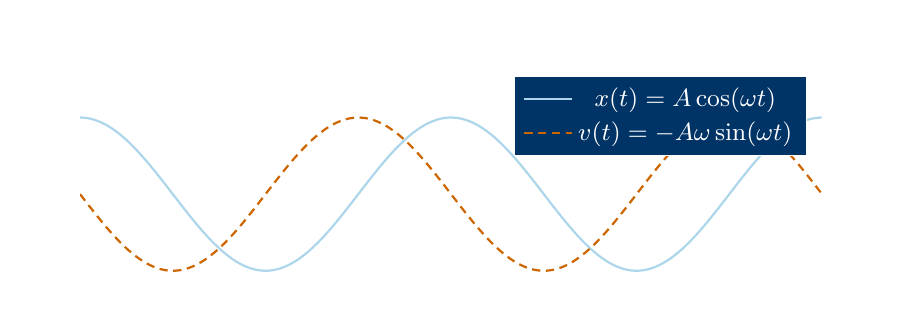
\begin{tikzpicture}
    \begin{axis}[
      width=11cm, height=4.5cm,
      axis lines=center,
      xlabel={$t\;[\text{s}]$},
      ylabel={$x(t)\;[\text{m}]$},
      xlabel style={right, font=\small\color{white}},
      ylabel style={above, font=\small\color{white}},
      tick style={color=white},
      ticklabel style={color=white, font=\tiny},
      axis line style={color=white, thick},
      xmin=0, xmax=12.56, ymin=-1.4, ymax=1.6,
      xtick=\empty, ytick=\empty,
      legend style={fill=NavyBlue, draw=white,
                    text=white, font=\small},
    ]
    \addplot[domain=0:4*pi, samples=300, thick, color=LightBlue]
      {cos(deg(x))};
    \addplot[domain=0:4*pi, samples=300, thick, color=AccentOrange,
             densely dashed]
      {-sin(deg(x))};
    \addlegendentry{$x(t)=A\cos(\omega t)$}
    \addlegendentry{$v(t)=-A\omega\sin(\omega t)$}
    \end{axis}
  \end{tikzpicture}

  \vspace{2.2cm}

  \begin{tabular}{rl}
    \textbf{Profesor:}    & Msc.\ N\'estor Fabio Montoya Palacios \\[5pt]
    \textbf{Asignatura:}  & F\'isica 3 \\[5pt]
    \textbf{Instituci\'on:} & Universidad Tecnol\'ogica de Pereira \\[5pt]
    \textbf{Fecha:}       & \today
  \end{tabular}

  \vfill
  {\small\sffamily\itshape
   ``La f\'isica es la b\'usqueda de la unidad en la diversidad'' \textemdash{} Abdus Salam}
\end{titlepage}
\pagecolor{white}\color{black}

%══════════════════════════════════════════════
%  TABLA DE CONTENIDOS
%══════════════════════════════════════════════
\tableofcontents
\clearpage

%══════════════════════════════════════════════
%  PRESENTACIÓN
%══════════════════════════════════════════════
\chapter*{Presentaci\'on}
\addcontentsline{toc}{chapter}{Presentaci\'on}

Este documento presenta la \textbf{soluci\'on completa y detallada} del taller de
\emph{Movimiento Arm\'onico Simple} (MAS) correspondiente a la asignatura
\textbf{F\'isica~3} de la Universidad Tecnol\'ogica de Pereira.

Cada problema es abordado con rigor matem\'atico: se identifican las magnitudes
relevantes, se aplican los principios f\'isicos pertinentes, se desarrolla el \'algebra
paso a paso y se enuncia claramente el resultado final en un recuadro.
Donde corresponde, se incluye c\'odigo en \textbf{Python} y \textbf{MATLAB}
como complemento num\'erico-gr\'afico.

\medskip
\begin{nota}
Las f\'ormulas fundamentales del MAS usadas en el taller son:
\[
  x(t) = A\cos(\omega t + \varphi),\qquad
  \omega = \sqrt{\dfrac{k}{m}},\qquad
  T = \dfrac{2\pi}{\omega},\qquad
  f = \dfrac{\omega}{2\pi}
\]
\[
  E = \tfrac{1}{2}kA^{2},\qquad
  v_{\max} = \omega A,\qquad
  a_{\max} = \omega^{2}A,\qquad
  U_{k} = \tfrac{1}{2}kx^{2},\qquad
  E_{c} = \tfrac{1}{2}mv^{2}
\]
\end{nota}

%══════════════════════════════════════════════
\chapter{Par\'ametros b\'asicos del MAS}
%══════════════════════════════════════════════

\section{Per\'iodo, frecuencia y amplitud}

%──────────────────────────────────
% Problema 1
\begin{problema}[title={Problema~1}]
Un resorte tiene una constante $k = 200\Nm$ y una masa de $m = 0{,}5\kg$ oscila en \'el.
?`Cu\'al es el \textbf{per\'iodo} de oscilaci\'on?
\end{problema}

\begin{solucion}
\textbf{Datos:} $k = 200\Nm$, $m = 0{,}5\kg$.

La frecuencia angular del sistema masa--resorte:
\[
  \omega = \sqrt{\dfrac{k}{m}} = \sqrt{\dfrac{200}{0{,}5}} = \sqrt{400} = 20\rad
\]

El per\'iodo de oscilaci\'on:
\[
  \boxed{T = \dfrac{2\pi}{\omega} = \dfrac{2\pi}{20} \approx 0{,}314\,\text{s}}
\]

\begin{center}
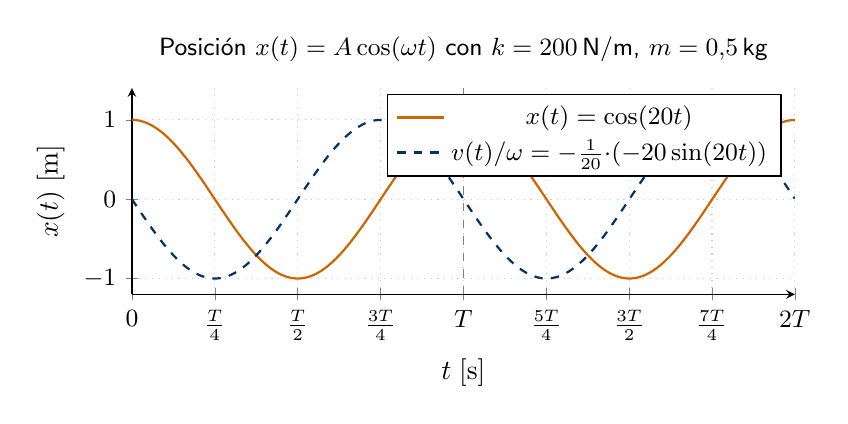
\begin{tikzpicture}
\begin{axis}[
  width=10cm, height=4.2cm,
  xlabel={$t\;[\text{s}]$}, ylabel={$x(t)\;[\text{m}]$},
  xmin=0, xmax=0.628, ymin=-1.2, ymax=1.4,
  xtick={0,0.0785,0.157,0.2355,0.314,0.3925,0.471,0.5495,0.628},
  xticklabels={$0$,$\frac{T}{4}$,$\frac{T}{2}$,$\frac{3T}{4}$,$T$,
               $\frac{5T}{4}$,$\frac{3T}{2}$,$\frac{7T}{4}$,$2T$},
  axis lines=left, grid=both, grid style={dotted, gray!40},
  tick label style={font=\small},
  title style={font=\small\sffamily},
  title={Posici\'on $x(t)=A\cos(\omega t)$ con $k=200\,\text{N/m}$, $m=0{,}5\,\text{kg}$},
  legend style={at={(0.98,0.97)}, anchor=north east, font=\small},
]
\addplot[domain=0:0.628, samples=300, thick, color=AccentOrange]
  {cos(deg(20*x))};
\addlegendentry{$x(t)=\cos(20t)$}
\addplot[domain=0:0.628, samples=300, thick, color=NavyBlue, dashed]
  {-sin(deg(20*x))};
\addlegendentry{$v(t)/\omega=-\tfrac{1}{20}{\cdot}(-20\sin(20t))$}
\draw[dashed, gray] (axis cs:0.314,-1.2) -- (axis cs:0.314,1.4)
  node[above, font=\tiny, gray]{$T$};
\end{axis}
\end{tikzpicture}
\end{center}
\end{solucion}

%──────────────────────────────────
% Problema 2
\begin{problema}[title={Problema~2}]
Encuentra la \textbf{amplitud} de un oscilador arm\'onico simple si la energ\'ia total
es $E = 2\,\text{J}$ y la constante del resorte es $k = 50\Nm$.
\end{problema}

\begin{solucion}
\textbf{Datos:} $E = 2\,\text{J}$, $k = 50\Nm$.

De la energ\'ia mec\'anica total $E = \tfrac{1}{2}kA^{2}$, despejando $A$:
\[
  A = \sqrt{\dfrac{2E}{k}} = \sqrt{\dfrac{2 \times 2}{50}} = \sqrt{0{,}08}
\]
\[
  \boxed{A \approx 0{,}283\,\text{m}}
\]
\end{solucion}

%──────────────────────────────────
% Problema 3
\begin{problema}[title={Problema~3}]
Determina la \textbf{frecuencia} de un p\'endulo simple de longitud $L = 2\mts$.
\end{problema}

\begin{solucion}
\textbf{Datos:} $L = 2\mts$, $g = 9{,}8\mss$.

Para oscilaciones de peque\~na amplitud:
\[
  \omega = \sqrt{\dfrac{g}{L}} = \sqrt{\dfrac{9{,}8}{2}} \approx 2{,}214\rad
\]
\[
  \boxed{f = \dfrac{\omega}{2\pi} \approx 0{,}352\Hz}
\]

\begin{center}
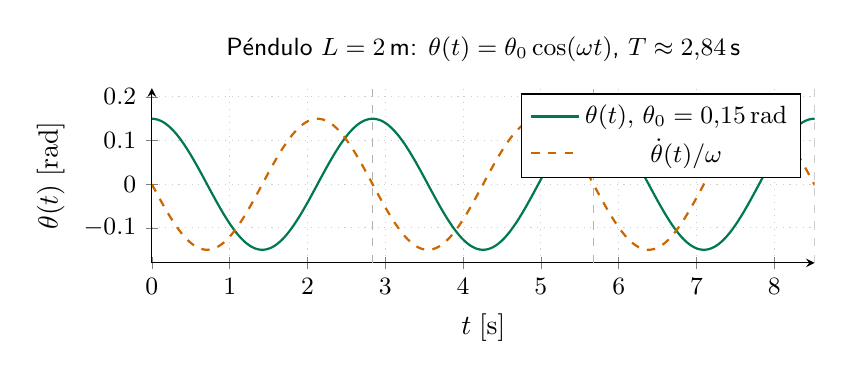
\begin{tikzpicture}
\begin{axis}[
  width=10cm, height=3.8cm,
  xlabel={$t\;[\text{s}]$}, ylabel={$\theta(t)\;[\text{rad}]$},
  xmin=0, xmax=8.52, ymin=-0.18, ymax=0.22,
  axis lines=left, grid=both, grid style={dotted,gray!40},
  tick label style={font=\small},
  title style={font=\small\sffamily},
  title={P\'endulo $L=2\,\text{m}$: $\theta(t)=\theta_0\cos(\omega t)$, $T\approx2{,}84\,\text{s}$},
  legend style={at={(0.98,0.97)}, anchor=north east, font=\small},
]
\addplot[domain=0:8.52, samples=400, thick, color=AccentGreen]
  {0.15*cos(deg(2.214*x))};
\addlegendentry{$\theta(t)$, $\theta_0=0{,}15\,\text{rad}$}
\addplot[domain=0:8.52, samples=400, thick, color=AccentOrange, dashed]
  {-0.15*sin(deg(2.214*x))};
\addlegendentry{$\dot\theta(t)/\omega$}
\draw[dashed,gray!60] (axis cs:2.838,-0.18) -- (axis cs:2.838,0.22);
\draw[dashed,gray!60] (axis cs:5.676,-0.18) -- (axis cs:5.676,0.22);
\draw[dashed,gray!60] (axis cs:8.514,-0.18) -- (axis cs:8.514,0.22);
\end{axis}
\end{tikzpicture}
\end{center}
\end{solucion}

%──────────────────────────────────
% Problema 4
\begin{problema}[title={Problema~4}]
Calcula la \textbf{energ\'ia cin\'etica m\'axima} de un oscilador arm\'onico simple
con $m = 1\kg$, $A = 0{,}1\mts$ y $\omega = 2\pi\rad$.
\end{problema}

\begin{solucion}
\textbf{Datos:} $m = 1\kg$, $A = 0{,}1\mts$, $\omega = 2\pi\rad$.

La energ\'ia cin\'etica m\'axima coincide con la energ\'ia total (posici\'on de equilibrio):
\[
  K_{\max} = \dfrac{1}{2}m\omega^{2}A^{2}
           = \dfrac{1}{2}(1)(2\pi)^{2}(0{,}1)^{2}
           = 0{,}02\pi^{2}
\]
\[
  \boxed{K_{\max} \approx 0{,}197\,\text{J}}
\]
\end{solucion}

%──────────────────────────────────
% Problema 5
\begin{problema}[title={Problema~5}]
Convierte la ecuaci\'on $x(t) = 0{,}05\cos\!\bigl(10t + \tfrac{\pi}{4}\bigr)$
al formato est\'andar $x(t) = A\cos(\omega t + \varphi)$ e identifica $A$,
$\omega$ y $\varphi$.
\end{problema}

\begin{solucion}
La ecuaci\'on ya est\'a en forma can\'onica del MAS. Por inspecci\'on directa:

\medskip
\begin{center}
\renewcommand{\arraystretch}{1.5}
\begin{tabular}{lll}
\toprule
Par\'ametro & S\'imbolo & Valor \\
\midrule
Amplitud            & $A$       & $0{,}05\,\text{m}$            \\
Frecuencia angular  & $\omega$  & $10\,\text{rad/s}$            \\
Fase inicial        & $\varphi$ & $\pi/4\,\text{rad} = 45^\circ$ \\
\bottomrule
\end{tabular}
\end{center}

\medskip
Magnitudes derivadas: $T = 2\pi/10 \approx 0{,}628\,\text{s}$,
$f \approx 1{,}592\Hz$.
\end{solucion}

%══════════════════════════════════════════════
\chapter{Simulaciones computacionales}
%══════════════════════════════════════════════

\section{Simulaci\'on del movimiento}

%──────────────────────────────────
% Problema 6
\begin{problema}[title={Problema~6}]
Utiliza \textbf{Python} para simular un MAS con $A = 1\mts$,
$\omega = 2\pi\rad$ y $\varphi = 0$. Grafica posici\'on, velocidad y aceleraci\'on.
\end{problema}

\begin{solucion}
Las ecuaciones del movimiento son:
\[
  x(t) = \cos(2\pi t),\quad
  v(t) = -2\pi\sin(2\pi t),\quad
  a(t) = -4\pi^{2}\cos(2\pi t)
\]

\begin{lstlisting}[caption={Simulaci\'on MAS en Python --- Problema 6}]
import numpy as np
import matplotlib.pyplot as plt

A, omega, phi = 1.0, 2*np.pi, 0.0
t = np.linspace(0, 2, 1000)  # 2 periodos

x = A * np.cos(omega*t + phi)
v = -A * omega * np.sin(omega*t + phi)
a = -A * omega**2 * np.cos(omega*t + phi)

fig, axes = plt.subplots(3, 1, figsize=(10, 8), sharex=True)
etiquetas = ['x(t) [m]', 'v(t) [m/s]', 'a(t) [m/s^2]']
datos     = [x, v, a]
colores   = ['royalblue', 'tomato', 'seagreen']

for ax, y, lbl, col in zip(axes, datos, etiquetas, colores):
    ax.plot(t, y, color=col, lw=2)
    ax.set_ylabel(lbl, fontsize=11)
    ax.axhline(0, color='k', lw=0.7, ls='--')
    ax.grid(alpha=0.3)

axes[-1].set_xlabel('Tiempo [s]', fontsize=11)
fig.suptitle('MAS -- Python', fontsize=13)
plt.tight_layout()
plt.show()
\end{lstlisting}

\begin{resultado}
Amplitudes m\'aximas:
$x_{\max} = 1\mts$,
$v_{\max} = 2\pi \approx 6{,}28\ms$,
$a_{\max} = 4\pi^{2} \approx 39{,}48\mss$.
\end{resultado}
\end{solucion}

%──────────────────────────────────
% Problema 7
\begin{problema}[title={Problema~7}]
Utiliza \textbf{MATLAB} para resolver la ecuaci\'on diferencial del MAS y graficar
el movimiento con los mismos par\'ametros.
\end{problema}

\begin{solucion}
\begin{lstlisting}[style=matlab, caption={Simulaci\'on MAS en MATLAB --- Problema 7}]
A = 1; omega = 2*pi;
t = linspace(0, 2, 1000);

x =  A * cos(omega*t);
v = -A * omega * sin(omega*t);
a = -A * omega^2 * cos(omega*t);

figure('Position',[100 100 900 700]);
tiledlayout(3,1)
nexttile; plot(t,x,'b','LineWidth',1.8); ylabel('x(t) [m]');   grid on;
nexttile; plot(t,v,'r','LineWidth',1.8); ylabel('v(t) [m/s]'); grid on;
nexttile; plot(t,a,'g','LineWidth',1.8); ylabel('a(t) [m/s2]');
          xlabel('Tiempo [s]'); grid on;
sgtitle('MAS -- MATLAB')
\end{lstlisting}
Los resultados num\'ericos son id\'enticos al Problema~6.
\end{solucion}

%══════════════════════════════════════════════
\chapter{Cinem\'atica del MAS}
%══════════════════════════════════════════════

\section{Velocidad, posici\'on y energ\'ia}

%──────────────────────────────────
% Problema 8
\begin{problema}[title={Problema~8}]
Determina el \textbf{tiempo} que tarda en alcanzar la velocidad m\'axima un objeto
en MAS con $A = 0{,}1\mts$ y $\omega = 5\rad$. Condici\'on inicial: $\varphi = 0$.
\end{problema}

\begin{solucion}
La velocidad es $v(t) = -A\omega\sin(\omega t)$.  
Es m\'axima cuando $|\sin(\omega t)| = 1$, es decir, $\omega t = \pi/2$:
\[
  t_{\max} = \dfrac{\pi/2}{\omega} = \dfrac{\pi}{2 \times 5} = \dfrac{\pi}{10}
\]
\[
  \boxed{t_{\max} \approx 0{,}314\,\text{s}}
\]
Corresponde al primer paso por la posici\'on de equilibrio ($x = 0$).

\begin{center}
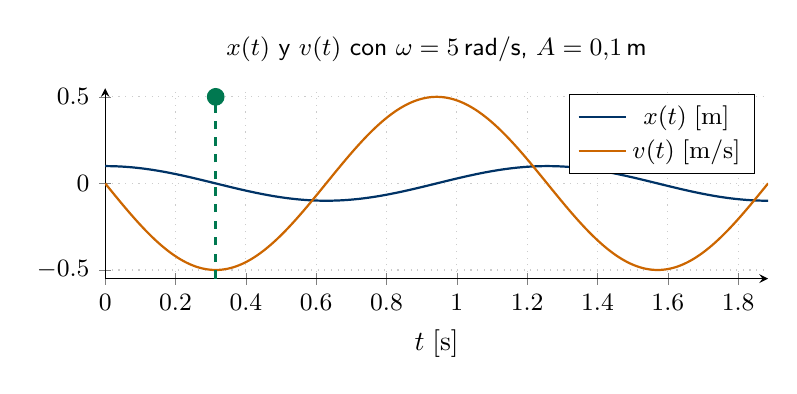
\begin{tikzpicture}
\begin{axis}[
  width=10cm, height=4cm,
  xlabel={$t\;[\text{s}]$},
  xmin=0, xmax=1.885, ymin=-0.55, ymax=0.55,
  axis lines=left, grid=both, grid style={dotted,gray!40},
  tick label style={font=\small},
  title style={font=\small\sffamily},
  title={$x(t)$ y $v(t)$ con $\omega=5\,\text{rad/s}$, $A=0{,}1\,\text{m}$},
  legend style={at={(0.98,0.97)}, anchor=north east, font=\small},
]
\addplot[domain=0:1.885, samples=400, thick, color=NavyBlue]
  {0.1*cos(deg(5*x))};
\addlegendentry{$x(t)\;[\text{m}]$}
\addplot[domain=0:1.885, samples=400, thick, color=AccentOrange]
  {-0.5*sin(deg(5*x))};
\addlegendentry{$v(t)\;[\text{m/s}]$}
\draw[very thick, AccentGreen, dashed]
  (axis cs:0.3142,-0.55) -- (axis cs:0.3142,0.55)
  node[above, font=\tiny\bfseries, AccentGreen]{$t_{\max}\!\approx\!0{,}314\,\text{s}$};
\addplot[only marks, mark=*, mark size=3pt, color=AccentGreen]
  coordinates {(0.3142, 0.5)};
\end{axis}
\end{tikzpicture}
\end{center}
\end{solucion}

%──────────────────────────────────
% Problema 9
\begin{problema}[title={Problema~9}]
Encuentra la \textbf{energ\'ia total} de un oscilador con $m = 2\kg$,
$k = 100\Nm$ y $A = 0{,}05\mts$.
\end{problema}

\begin{solucion}
\[
  E = \dfrac{1}{2}kA^{2} = \dfrac{1}{2}(100)(0{,}05)^{2} = \dfrac{1}{2}(100)(0{,}0025)
\]
\[
  \boxed{E = 0{,}125\,\text{J}}
\]
\end{solucion}

%──────────────────────────────────
% Problema 10
\begin{problema}[title={Problema~10}]
Calcula la \textbf{posici\'on} en $t = 2\,\text{s}$ para $x_{0} = 0{,}1\mts$,
$v_{0} = 0$ y $\omega = 4\rad$.
\end{problema}

\begin{solucion}
Con $v_{0} = 0$, la soluci\'on es $x(t) = x_{0}\cos(\omega t)$:
\[
  x(2) = 0{,}1\cos(4 \times 2) = 0{,}1\cos(8\,\text{rad})
\]
\[
  \boxed{x(2) \approx -0{,}099\,\text{m}}
\]
\end{solucion}

%══════════════════════════════════════════════
\chapter{Gr\'aficas de energ\'ia}
%══════════════════════════════════════════════

\section{Energ\'ia cin\'etica, potencial y total}

%──────────────────────────────────
% Problema 11
\begin{problema}[title={Problema~11}]
Utiliza \textbf{Python} para graficar $E_c$, $U_k$ y $E$ de un MAS con
$A = 1\mts$, $\omega = 2\pi\rad$, $m = 1\kg$.
\end{problema}

\begin{solucion}
\begin{lstlisting}[caption={Gr\'aficas de energ\'ia MAS --- Problema 11}]
import numpy as np
import matplotlib.pyplot as plt

A, omega, m = 1.0, 2*np.pi, 1.0
k = m * omega**2
t = np.linspace(0, 2, 1000)

x  = A * np.cos(omega*t)
v  = -A * omega * np.sin(omega*t)
Uk = 0.5*k*x**2
Ec = 0.5*m*v**2
E  = np.full_like(t, 0.5*k*A**2)

plt.figure(figsize=(10, 5))
plt.plot(t, Uk, 'b',  lw=2, label='$U_k$ (potencial)')
plt.plot(t, Ec, 'r',  lw=2, label='$E_c$ (cinetica)')
plt.plot(t, E,  'k--',lw=2, label='$E$ (total)')
plt.xlabel('Tiempo [s]'); plt.ylabel('Energia [J]')
plt.title('Energias del MAS'); plt.legend(); plt.grid(alpha=0.3)
plt.tight_layout(); plt.show()
\end{lstlisting}

\medskip
\textbf{Gr\'afica anal\'itica con pgfplots} ($A=1\,\text{m}$, $\omega=2\pi\,\text{rad/s}$,
$m=1\,\text{kg}$, $k=4\pi^{2}\,\text{N/m}$, $E=2\pi^{2}\approx19{,}74\,\text{J}$):

\begin{center}
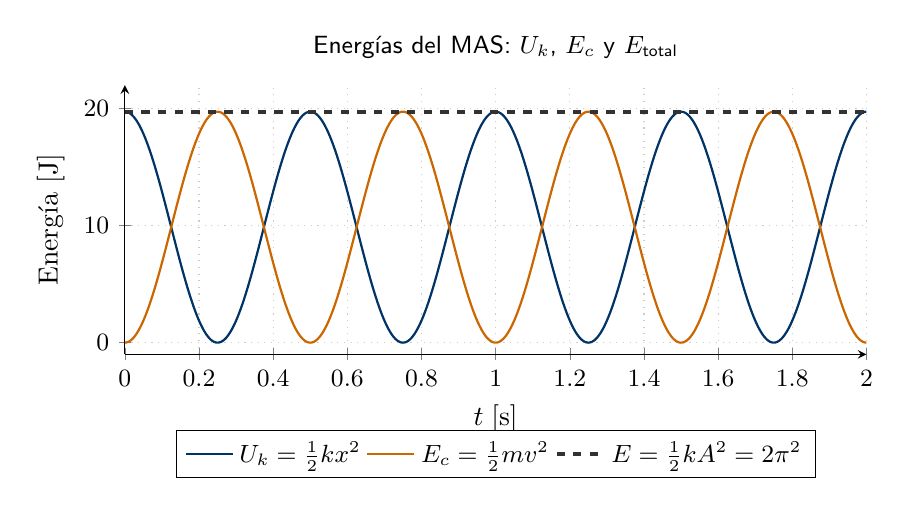
\begin{tikzpicture}
\begin{axis}[
  width=11cm, height=5cm,
  xlabel={$t\;[\text{s}]$}, ylabel={Energ\'ia $[\text{J}]$},
  xmin=0, xmax=2, ymin=-1, ymax=22,
  axis lines=left, grid=both, grid style={dotted,gray!40},
  tick label style={font=\small},
  title style={font=\small\sffamily},
  title={Energ\'ias del MAS: $U_k$, $E_c$ y $E_{\text{total}}$},
  legend style={at={(0.5,-0.28)}, anchor=north, legend columns=3, font=\small},
]
\addplot[domain=0:2, samples=500, thick, color=NavyBlue]
  {19.7392*cos(deg(2*pi*x))^2};
\addlegendentry{$U_k = \tfrac{1}{2}k x^2$}
\addplot[domain=0:2, samples=500, thick, color=AccentOrange]
  {19.7392*sin(deg(2*pi*x))^2};
\addlegendentry{$E_c = \tfrac{1}{2}mv^2$}
\addplot[domain=0:2, samples=10, thick, color=DarkGray, dashed, line width=1.5pt]
  {19.7392};
\addlegendentry{$E = \tfrac{1}{2}kA^2 = 2\pi^2$}
\end{axis}
\end{tikzpicture}
\end{center}

\begin{resultado}
$E_{\text{total}} = \tfrac{1}{2}kA^{2} = 2\pi^{2} \approx 19{,}74\,\text{J}$.\\
$U_k$ y $E_c$ oscilan en antifase con frecuencia $2\omega$; su suma es constante.
\end{resultado}
\end{solucion}

%──────────────────────────────────
% Problema 12
\begin{problema}[title={Problema~12}]
Utiliza \textbf{MATLAB} para las mismas gr\'aficas de energ\'ia.
\end{problema}

\begin{solucion}
\begin{lstlisting}[style=matlab, caption={Gr\'aficas de energ\'ia --- Problema 12}]
A=1; omega=2*pi; m=1; k=m*omega^2;
t=linspace(0,2,1000);
x=A*cos(omega*t); v=-A*omega*sin(omega*t);
Uk=0.5*k*x.^2; Ec=0.5*m*v.^2;
E=0.5*k*A^2*ones(size(t));

figure; hold on;
plot(t,Uk,'b','LineWidth',2,'DisplayName','U_k');
plot(t,Ec,'r','LineWidth',2,'DisplayName','E_c');
plot(t,E,'k--','LineWidth',2,'DisplayName','E total');
xlabel('Tiempo [s]'); ylabel('Energia [J]');
title('Energias del MAS'); legend; grid on;
\end{lstlisting}
\end{solucion}

%══════════════════════════════════════════════
\chapter{Problemas de textos cl\'asicos}
%══════════════════════════════════════════════

\section{Serway, Sears-Zemansky y Bauer}

%──────────────────────────────────
% Problema 13
\begin{problema}[title={Problema~13 --- Serway}]
Un bloque de masa $m$ unido a un resorte de constante $k$ oscila sin fricci\'on.
Se desplaza $A$ y se suelta ($v_{0}=0$). ?`Cu\'al es la \textbf{velocidad m\'axima}?
\end{problema}

\begin{solucion}
Por conservaci\'on de energ\'ia entre el extremo ($x=A$, $v=0$) y el equilibrio
($x=0$, $v=v_{\max}$):
\[
  \dfrac{1}{2}kA^{2} = \dfrac{1}{2}mv_{\max}^{2}
  \implies
  \boxed{v_{\max} = A\sqrt{\dfrac{k}{m}} = \omega A}
\]
\end{solucion}

%──────────────────────────────────
% Problema 14
\begin{problema}[title={Problema~14 --- Sears \& Zemansky}]
Un p\'endulo simple de longitud $L$ y masa $m$ se desplaza desde $\theta_{0}$.
Determina la \textbf{velocidad m\'axima}.
\end{problema}

\begin{solucion}
La altura respecto al equilibrio es $h = L(1-\cos\theta_{0})$.
Por conservaci\'on de energ\'ia:
\[
  \dfrac{1}{2}mv_{\max}^{2} = mgL(1-\cos\theta_{0})
\]
\[
  \boxed{v_{\max} = \sqrt{2gL(1-\cos\theta_{0})}}
\]

\begin{nota}
Para $\theta_{0}\ll 1$: $v_{\max} \approx \theta_{0}\sqrt{gL}$, consistente
con $v_{\max} = \omega A$ del MAS ($\omega = \sqrt{g/L}$, $A = L\theta_{0}$).
\end{nota}
\end{solucion}

%──────────────────────────────────
% Problema 15
\begin{problema}[title={Problema~15 --- Bauer}]
Una part\'icula sujeta a $F=-kx$ con energ\'ia total $E$.
Determina la \textbf{amplitud}.
\end{problema}

\begin{solucion}
\[
  E = \dfrac{1}{2}kA^{2}
  \implies
  \boxed{A = \sqrt{\dfrac{2E}{k}}}
\]
\textbf{Verificaci\'on dimensional:}
$[A] = \sqrt{\text{J}/(\text{N/m})} = \sqrt{\text{m}^{2}} = \text{m}$ \checkmark
\end{solucion}

%══════════════════════════════════════════════
\chapter{An\'alisis de par\'ametros}
%══════════════════════════════════════════════

\section{Efecto de $\omega$ y de la amplitud $A$}

%──────────────────────────────────
% Problema 16
\begin{problema}[title={Problema~16}]
Compara las gr\'aficas de $E_c$ y $U_k$ de un MAS con diferentes valores de $\omega$.
\end{problema}

\begin{solucion}
Las energ\'ias en funci\'on del tiempo (con $\varphi = 0$):
\[
  U_{k}(t) = \dfrac{E}{2}\bigl[1+\cos(2\omega t)\bigr],\qquad
  E_{c}(t) = \dfrac{E}{2}\bigl[1-\cos(2\omega t)\bigr]
\]

Ambas oscilan con frecuencia angular $\Omega = 2\omega$ (el doble del movimiento).

\medskip
\begin{center}
\renewcommand{\arraystretch}{1.4}
\begin{tabular}{ccc}
\toprule
$\omega\;[\text{rad/s}]$ & $\Omega = 2\omega\;[\text{rad/s}]$ &
$T_{\text{energ.}} = \pi/\omega\;[\text{s}]$ \\
\midrule
$1$     & $2$     & $3{,}14$  \\
$2\pi$  & $4\pi$  & $0{,}50$  \\
$10$    & $20$    & $0{,}31$  \\
\bottomrule
\end{tabular}
\end{center}

\medskip
\textbf{Comparaci\'on gr\'afica} para $A=1\,\text{m}$, $m=1\,\text{kg}$ y tres
valores de $\omega$:

\begin{center}
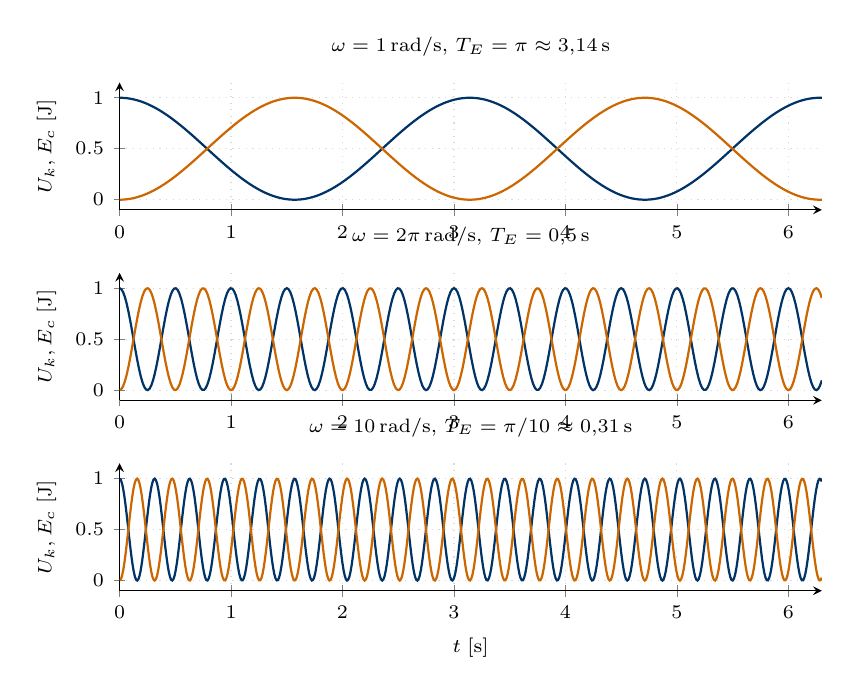
\begin{tikzpicture}
\begin{groupplot}[
  group style={group size=1 by 3, vertical sep=0.8cm},
  width=10.5cm, height=3.2cm,
  axis lines=left, grid=both, grid style={dotted,gray!30},
  xmin=0, xmax=6.3, ymin=-0.1, ymax=1.15,
  tick label style={font=\scriptsize},
  ylabel style={font=\scriptsize},
  xlabel style={font=\scriptsize},
]
\nextgroupplot[title={\scriptsize$\omega=1\,\text{rad/s}$, $T_E=\pi\approx3{,}14\,\text{s}$},
               ylabel={$U_k,E_c\;[\text{J}]$}]
  \addplot[domain=0:6.3,samples=300,thick,color=NavyBlue]{0.5*(1+cos(deg(2*x)))};
  \addplot[domain=0:6.3,samples=300,thick,color=AccentOrange]{0.5*(1-cos(deg(2*x)))};
\nextgroupplot[title={\scriptsize$\omega=2\pi\,\text{rad/s}$, $T_E=0{,}5\,\text{s}$},
               ylabel={$U_k,E_c\;[\text{J}]$}]
  \addplot[domain=0:6.3,samples=400,thick,color=NavyBlue]{0.5*(1+cos(deg(4*pi*x)))};
  \addplot[domain=0:6.3,samples=400,thick,color=AccentOrange]{0.5*(1-cos(deg(4*pi*x)))};
\nextgroupplot[title={\scriptsize$\omega=10\,\text{rad/s}$, $T_E=\pi/10\approx0{,}31\,\text{s}$},
               ylabel={$U_k,E_c\;[\text{J}]$}, xlabel={$t\;[\text{s}]$}]
  \addplot[domain=0:6.3,samples=600,thick,color=NavyBlue]{0.5*(1+cos(deg(20*x)))};
  \addplot[domain=0:6.3,samples=600,thick,color=AccentOrange]{0.5*(1-cos(deg(20*x)))};
\end{groupplot}
\end{tikzpicture}
\end{center}
{\footnotesize\color{NavyBlue}$\blacksquare$\ $U_k$\hspace{1em}\color{AccentOrange}$\blacksquare$\ $E_c$}

\textbf{Conclusi\'on:} Mayor $\omega$ implica intercambio energ\'etico m\'as r\'apido;
la energ\'ia total $E = \tfrac{1}{2}kA^{2}$ crece con $k=m\omega^{2}$ si $A$ se mantiene fija.
\end{solucion}

%──────────────────────────────────
% Problema 17
\begin{problema}[title={Problema~17}]
Analiza el \textbf{efecto de la amplitud} $A$ en la energ\'ia total de un MAS.
\end{problema}

\begin{solucion}
$E = \tfrac{1}{2}kA^{2}$: la relaci\'on es \textbf{cuadr\'atica}.

\begin{center}
\renewcommand{\arraystretch}{1.4}
\begin{tabular}{ccc}
\toprule
$A$ & $E = \tfrac{1}{2}kA^{2}$ & Factor \\
\midrule
$A_{0}$  & $\tfrac{1}{2}kA_{0}^{2}$      & $1\times$   \\
$2A_{0}$ & $2kA_{0}^{2}$                  & $4\times$   \\
$3A_{0}$ & $\tfrac{9}{2}kA_{0}^{2}$       & $9\times$   \\
$nA_{0}$ & $\tfrac{n^{2}}{2}kA_{0}^{2}$   & $n^{2}\times$ \\
\bottomrule
\end{tabular}
\end{center}

\begin{center}
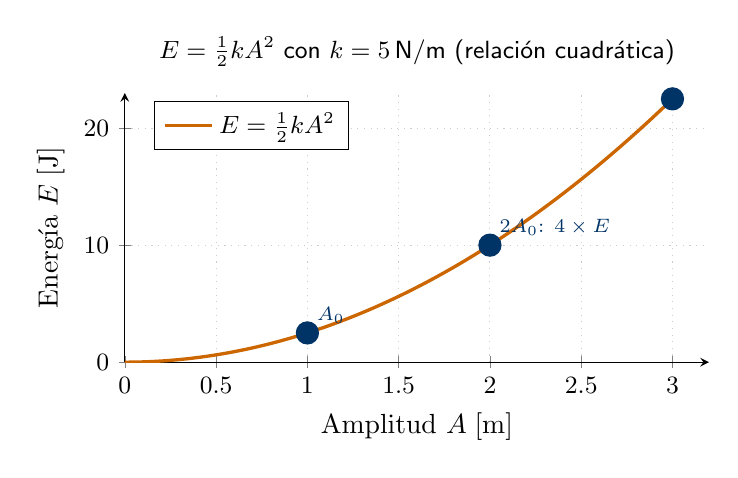
\begin{tikzpicture}
\begin{axis}[
  width=9cm, height=5cm,
  xlabel={Amplitud $A\;[\text{m}]$}, ylabel={Energ\'ia $E\;[\text{J}]$},
  xmin=0, xmax=3.2, ymin=0, ymax=23,
  axis lines=left, grid=both, grid style={dotted,gray!40},
  tick label style={font=\small},
  title style={font=\small\sffamily},
  title={$E=\tfrac{1}{2}kA^2$ con $k=5\,\text{N/m}$ (relaci\'on cuadr\'atica)},
  legend style={at={(0.05,0.97)}, anchor=north west, font=\small},
]
\addplot[domain=0:3, samples=200, very thick, color=AccentOrange]
  {2.5*x^2};
\addlegendentry{$E=\tfrac{1}{2}kA^2$}
\addplot[only marks, mark=*, mark size=4pt, color=NavyBlue]
  coordinates {(1,2.5)(2,10)(3,22.5)};
\node[font=\scriptsize, NavyBlue, above right] at (axis cs:1,2.5) {$A_0$};
\node[font=\scriptsize, NavyBlue, above right] at (axis cs:2,10) {$2A_0$: $4\times E$};
\node[font=\scriptsize, NavyBlue, above right] at (axis cs:3,22.5) {$3A_0$: $9\times E$};
\end{axis}
\end{tikzpicture}
\end{center}

\begin{resultado}
$E \propto A^{2}$: duplicar la amplitud \textbf{cuadruplica} la energ\'ia.
\end{resultado}
\end{solucion}

%══════════════════════════════════════════════
\chapter{MAS amortiguado y forzado}
%══════════════════════════════════════════════

\section{Nivel avanzado}

%──────────────────────────────────
% Problema 18
\begin{problema}[title={Problema~18 --- Nivel avanzado}]
Simula en Python un MAS con \textbf{amortiguamiento} y grafica posici\'on, velocidad
y aceleraci\'on.
\end{problema}

\begin{solucion}
La ecuaci\'on del oscilador amortiguado es:
\[
  \dddt{x} + 2\gamma\ddt{x} + \omega_{0}^{2}x = 0,\qquad
  \gamma = \dfrac{b}{2m},\quad \omega_{0} = \sqrt{\dfrac{k}{m}}
\]

Soluci\'on subamortiguada ($\gamma < \omega_{0}$):
\[
  x(t) = Ae^{-\gamma t}\cos(\omega_{d}t + \varphi),\qquad
  \omega_{d} = \sqrt{\omega_{0}^{2}-\gamma^{2}}
\]

\begin{lstlisting}[caption={MAS amortiguado --- Problema 18}]
import numpy as np
import matplotlib.pyplot as plt
from scipy.integrate import solve_ivp

m, k, b = 1.0, 100.0, 2.0
omega0 = np.sqrt(k/m); gamma = b/(2*m)
omega_d = np.sqrt(omega0**2 - gamma**2)

def ode(t, y):
    x, v = y
    return [v, -2*gamma*v - omega0**2*x]

sol = solve_ivp(ode, [0,10], [1.0,0.0],
                t_eval=np.linspace(0,10,2000))
t, x = sol.t, sol.y[0]
v = sol.y[1]
a = np.gradient(v, t)
env = np.exp(-gamma*t)

fig, axes = plt.subplots(3,1, figsize=(10,9), sharex=True)
for ax,y,lbl,col in zip(axes,[x,v,a],
    ['x(t)[m]','v(t)[m/s]','a(t)[m/s2]'],
    ['royalblue','tomato','seagreen']):
    ax.plot(t,y,color=col,lw=1.8); ax.set_ylabel(lbl); ax.grid(alpha=0.3)
axes[0].plot(t,env,'k--',lw=1.2,label='Envolvente')
axes[0].plot(t,-env,'k--',lw=1.2); axes[0].legend()
axes[-1].set_xlabel('Tiempo [s]')
fig.suptitle('MAS Amortiguado'); plt.tight_layout(); plt.show()
\end{lstlisting}

\begin{resultado}
Par\'ametros num\'ericos: $\omega_{0} = 10\rad$, $\gamma = 1\rad$,
$\omega_{d} = \sqrt{99} \approx 9{,}95\rad$. La amplitud decae como $e^{-t}$.
\end{resultado}

\medskip
\textbf{Gr\'afica anal\'itica} $x(t)=e^{-\gamma t}\cos(\omega_d t)$ con pgfplots:

\begin{center}
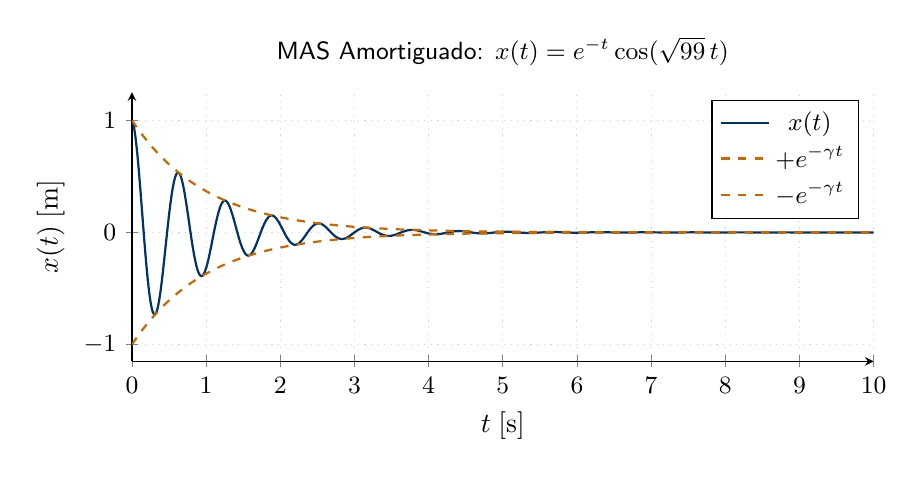
\begin{tikzpicture}
\begin{axis}[
  width=11cm, height=5cm,
  xlabel={$t\;[\text{s}]$}, ylabel={$x(t)\;[\text{m}]$},
  xmin=0, xmax=10, ymin=-1.15, ymax=1.25,
  axis lines=left, grid=both, grid style={dotted,gray!35},
  tick label style={font=\small},
  title style={font=\small\sffamily},
  title={MAS Amortiguado: $x(t)=e^{-t}\cos(\sqrt{99}\,t)$},
  legend style={at={(0.98,0.97)}, anchor=north east, font=\small},
]
\addplot[domain=0:10, samples=600, thick, color=NavyBlue]
  {exp(-x)*cos(deg(9.9499*x))};
\addlegendentry{$x(t)$}
\addplot[domain=0:10, samples=200, thick, color=AccentOrange, dashed]
  {exp(-x)};
\addlegendentry{$+e^{-\gamma t}$}
\addplot[domain=0:10, samples=200, thick, color=AccentOrange, dashed]
  {-exp(-x)};
\addlegendentry{$-e^{-\gamma t}$}
\end{axis}
\end{tikzpicture}
\end{center}
\end{solucion}

%──────────────────────────────────
% Problema 19
\begin{problema}[title={Problema~19 --- Nivel avanzado}]
Resuelve y grafica en MATLAB el MAS con \textbf{fuerza externa}
$F(t) = F_{0}\cos(\omega t)$.
\end{problema}

\begin{solucion}
La ecuaci\'on del oscilador forzado:
\[
  m\dddt{x} + b\ddt{x} + kx = F_{0}\cos(\omega t)
\]

Soluci\'on estacionaria:
\[
  x_{p}(t) = \dfrac{F_{0}/m}{\sqrt{(\omega_{0}^{2}-\omega^{2})^{2}+(2\gamma\omega)^{2}}}
             \cos(\omega t - \delta),\qquad
  \tan\delta = \dfrac{2\gamma\omega}{\omega_{0}^{2}-\omega^{2}}
\]

\begin{lstlisting}[style=matlab, caption={Oscilador forzado en MATLAB --- Problema 19}]
m=1; k=100; b=2; F0=10; omega=8;
ode_fun = @(t,y) [y(2);
    (F0*cos(omega*t) - b*y(2) - k*y(1))/m];
[t,y] = ode45(ode_fun, [0 20], [0;0]);
x=y(:,1); v=y(:,2);
a=(F0*cos(omega*t)-b*v-k*x)/m;

figure;
subplot(3,1,1); plot(t,x,'b','LineWidth',1.8);
  ylabel('x(t) [m]'); title('Posicion'); grid on;
subplot(3,1,2); plot(t,v,'r','LineWidth',1.8);
  ylabel('v(t) [m/s]'); title('Velocidad'); grid on;
subplot(3,1,3); plot(t,a,'g','LineWidth',1.8);
  ylabel('a(t) [m/s2]'); xlabel('Tiempo [s]'); grid on;
sgtitle('Oscilador Forzado')
\end{lstlisting}

\begin{nota}
En resonancia ($\omega = \omega_{0}$) la amplitud estacionaria es
$x_{\max} = F_{0}/(b\omega_{0})$.
\end{nota}
\end{solucion}

%══════════════════════════════════════════════
\chapter{Problemas adicionales de velocidad, energ\'ia y frecuencia}
%══════════════════════════════════════════════

\section{Velocidad m\'axima, energ\'ia y par\'ametros din\'amicos}

%──────────────────────────────────
% Problema 20
\begin{problema}[title={Problema~20}]
Un oscilador con $f = 5\Hz$ y $A = 0{,}2\mts$.
?`Cu\'al es la \textbf{velocidad m\'axima}?
\end{problema}

\begin{solucion}
\[
  \omega = 2\pi f = 10\pi\rad
\]
\[
  \boxed{v_{\max} = \omega A = 10\pi \times 0{,}2 = 2\pi \approx 6{,}28\ms}
\]
\end{solucion}

%──────────────────────────────────
% Problema 21
\begin{problema}[title={Problema~21}]
Energ\'ia total con $m = 3\kg$, $k = 120\Nm$, $A = 0{,}15\mts$.
\end{problema}

\begin{solucion}
\[
  \boxed{E = \dfrac{1}{2}kA^{2} = \dfrac{1}{2}(120)(0{,}15)^{2} = 1{,}35\,\text{J}}
\]
\end{solucion}

%──────────────────────────────────
% Problema 22
\begin{problema}[title={Problema~22}]
Aceleraci\'on m\'axima de un p\'endulo simple con $L = 1{,}5\mts$,
$\theta_{0} = 0{,}1\,\text{rad}$.
\end{problema}

\begin{solucion}
Para peque\~nas oscilaciones $a_{\max} = g\theta_{0}$:
\[
  \boxed{a_{\max} = 9{,}8 \times 0{,}1 = 0{,}98\mss}
\]
\end{solucion}

%──────────────────────────────────
% Problema 23
\begin{problema}[title={Problema~23}]
Simula el MAS en \textbf{GeoGebra} y describe el resultado.
\end{problema}

\begin{solucion}
En GeoGebra se puede modelar el MAS definiendo:
\[
  x(t) = A\cos(\omega t + \varphi)
\]
con deslizadores para $A$, $\omega$ y $\varphi$. La curva resultante es una
sinusoide cuya frecuencia y amplitud se controlan interactivamente.

\textbf{Observaciones din\'amicas:}
\begin{itemize}[leftmargin=*]
  \item Aumentar $A$ eleva la amplitud de la curva sin cambiar $T$.
  \item Aumentar $\omega$ comprime horizontalmente la curva (menor $T$).
  \item Cambiar $\varphi$ desplaza la curva horizontalmente.
\end{itemize}
\end{solucion}

%──────────────────────────────────
% Problema 24
\begin{problema}[title={Problema~24}]
Describe c\'omo var\'ia la energ\'ia total de un MAS con la amplitud.
\end{problema}

\begin{solucion}
$E = \tfrac{1}{2}kA^{2}$: la energ\'ia total es proporcional al \textbf{cuadrado}
de la amplitud. Doblar $A$ cuadruplica $E$. (Ver tabla en el Problema~17.)
\end{solucion}

%──────────────────────────────────
% Problema 25
\begin{problema}[title={Problema~25}]
Utiliza \textbf{Wolfram Alpha} para resolver la EDO del MAS.
\end{problema}

\begin{solucion}
Entrada en Wolfram Alpha:
\[
  \texttt{dsolve x''(t) + omega\^{}2 x(t) = 0}
\]
Respuesta: $x(t) = C_{1}\cos(\omega t) + C_{2}\sin(\omega t)$,
que con condiciones iniciales $x(0)=x_{0}$, $x'(0)=v_{0}$ da
$C_{1}=x_{0}$, $C_{2}=v_{0}/\omega$.
\end{solucion}

%──────────────────────────────────
% Problema 26
\begin{problema}[title={Problema~26}]
Explica el efecto de la fricci\'on en un sistema masa--resorte.
\end{problema}

\begin{solucion}
La fricci\'on introduce un t\'ermino de amortiguamiento $b\dot{x}$ en la EDO:
\[
  m\ddot{x} + b\dot{x} + kx = 0
\]

Dependiendo del factor $\zeta = b/(2\sqrt{km})$:

\begin{center}
\renewcommand{\arraystretch}{1.4}
\begin{tabular}{llp{6cm}}
\toprule
Caso & Condici\'on & Comportamiento \\
\midrule
Subamortiguado  & $\zeta < 1$ & Oscilaciones con amplitud decreciente ($e^{-\gamma t}$) \\
Cr\'iticamente amortiguado & $\zeta = 1$ & Retorno al equilibrio sin oscilaciones, m\'as r\'apido \\
Sobreamortiguado & $\zeta > 1$ & Retorno lento, sin oscilaciones \\
\bottomrule
\end{tabular}
\end{center}

\begin{center}
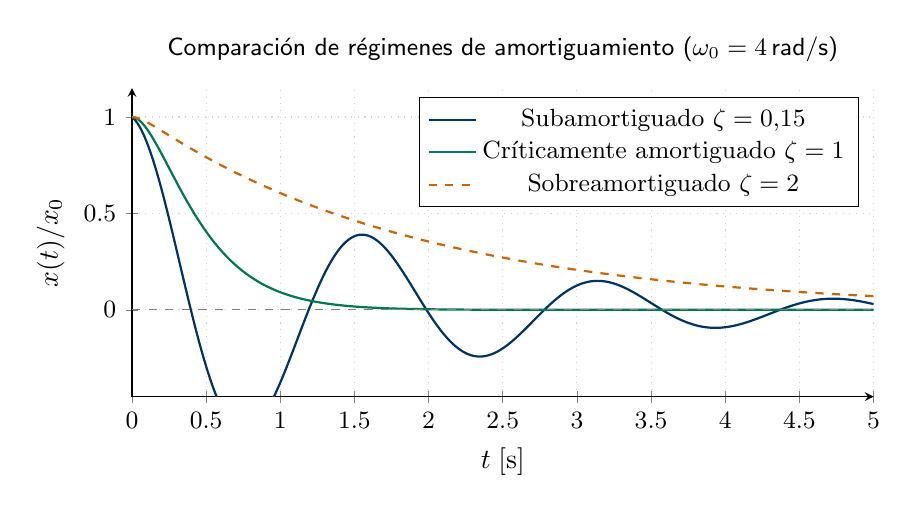
\begin{tikzpicture}
\begin{axis}[
  width=11cm, height=5.5cm,
  xlabel={$t\;[\text{s}]$}, ylabel={$x(t)/x_0$},
  xmin=0, xmax=5, ymin=-0.45, ymax=1.15,
  axis lines=left, grid=both, grid style={dotted,gray!35},
  tick label style={font=\small},
  title style={font=\small\sffamily},
  title={Comparaci\'on de r\'egimenes de amortiguamiento ($\omega_0=4\,\text{rad/s}$)},
  legend style={at={(0.98,0.97)}, anchor=north east, font=\small},
]
% Subamortiguado: zeta=0.15, gamma=0.6, omega_d=sqrt(16-0.36)=sqrt(15.64)=3.955
\addplot[domain=0:5, samples=400, thick, color=NavyBlue]
  {exp(-0.6*x)*cos(deg(3.955*x))};
\addlegendentry{Subamortiguado $\zeta=0{,}15$}
% Criticamente amortiguado: x(t)=(1+omega0*t)*exp(-omega0*t)
\addplot[domain=0:5, samples=300, thick, color=AccentGreen]
  {(1+4*x)*exp(-4*x)};
\addlegendentry{Cr\'iticamente amortiguado $\zeta=1$}
% Sobreamortiguado: zeta=2, r1=-8+sqrt(48)=-0.536, r2=-8-sqrt(48)=-15.46 (aprox)
\addplot[domain=0:5, samples=200, thick, color=AccentOrange, dashed]
  {1.035*exp(-0.536*x) - 0.035*exp(-15.46*x)};
\addlegendentry{Sobreamortiguado $\zeta=2$}
\draw[dashed, gray] (axis cs:0,0) -- (axis cs:5,0);
\end{axis}
\end{tikzpicture}
\end{center}
\end{solucion}

%──────────────────────────────────
% Problema 27
\begin{problema}[title={Problema~27}]
Encuentra la frecuencia natural con $k = 80\Nm$ y $m = 2\kg$.
\end{problema}

\begin{solucion}
\[
  \omega = \sqrt{\dfrac{80}{2}} = \sqrt{40} \approx 6{,}325\rad,\qquad
  \boxed{f = \dfrac{6{,}325}{2\pi} \approx 1{,}006\Hz}
\]
\end{solucion}

%──────────────────────────────────
% Problema 28
\begin{problema}[title={Problema~28}]
Per\'iodo de un resorte con $k = 250\Nm$ y $m = 0{,}75\kg$.
\end{problema}

\begin{solucion}
\[
  \omega = \sqrt{\dfrac{250}{0{,}75}} \approx 18{,}26\rad,\qquad
  \boxed{T \approx \dfrac{2\pi}{18{,}26} \approx 0{,}344\,\text{s}}
\]
\end{solucion}

%──────────────────────────────────
% Problema 29
\begin{problema}[title={Problema~29}]
Utiliza \textbf{Symbolab} para encontrar la soluci\'on general de la EDO del MAS.
\end{problema}

\begin{solucion}
Entrada en Symbolab: \texttt{d\^{}2x/dt\^{}2 + omega\^{}2 x = 0}.

Respuesta: $x(t) = C_{1}\cos(\omega t) + C_{2}\sin(\omega t)$, id\'entica
a la obtenida anal\'iticamente.
\end{solucion}

%──────────────────────────────────
% Problema 30
\begin{problema}[title={Problema~30}]
Compara las soluciones num\'ericas y anal\'iticas del MAS en MATLAB.
\end{problema}

\begin{solucion}
\begin{lstlisting}[style=matlab, caption={Comparaci\'on anal\'itica vs.\ num\'erica --- Problema 30}]
m=1; k=4; omega0=sqrt(k/m); x0=1; v0=0;
t_an = linspace(0,10,1000);
x_an = x0*cos(omega0*t_an);  % Solucion analitica

ode_fn = @(t,y) [y(2); -(k/m)*y(1)];
[t_num, y_num] = ode45(ode_fn,[0 10],[x0;v0]);
x_num = y_num(:,1);  % Solucion numerica

figure; hold on;
plot(t_an, x_an,'b-','LineWidth',2.5,'DisplayName','Analitica');
plot(t_num,x_num,'r--','LineWidth',1.5,'DisplayName','Numerica');
xlabel('t [s]'); ylabel('x(t) [m]');
title('MAS: Analitica vs Numerica'); legend; grid on;

err = max(abs(x_an - interp1(t_num,x_num,t_an)));
fprintf('Error maximo: %.2e m\n', err);
\end{lstlisting}

\begin{resultado}
El error m\'aximo entre soluciones es del orden $10^{-10}\,\text{m}$,
confirmando la precisi\'on del m\'etodo RK45.
\end{resultado}
\end{solucion}

%══════════════════════════════════════════════
\chapter{Problemas de Beer, Johnston \& Cornwell y Hibbeler}
%══════════════════════════════════════════════

\section{Din\'amica de sistemas con resortes y barras}

%──────────────────────────────────
% Problema 31
\begin{problema}[title={Problema~31 --- Beer, Johnston \& Cornwell (19.21)}]
Un bloque de $30\,\text{lb}$ oscila con amplitud $0{,}8\,\text{in}$ y
per\'iodo $T = 1{,}5\,\text{s}$. Determina:
\begin{enumerate}[label=\alph*)]
  \item La constante equivalente $k$.
  \item La velocidad y aceleraci\'on m\'aximas.
\end{enumerate}
\end{problema}

\begin{solucion}
\textbf{Conversi\'on:}
\[
  m = \dfrac{30\,\text{lb}}{32{,}2\,\text{ft/s}^{2}} \approx 0{,}932\,\text{slug},\qquad
  A = \dfrac{0{,}8}{12}\,\text{ft} \approx 0{,}0667\,\text{ft}
\]

\textbf{a) Constante $k$:}
\[
  T = 2\pi\sqrt{\dfrac{m}{k}}
  \implies
  k = m\!\left(\dfrac{2\pi}{T}\right)^{\!2}
    = 0{,}932 \times \left(\dfrac{2\pi}{1{,}5}\right)^{\!2}
    \approx 0{,}932 \times 17{,}546
\]
\[
  \boxed{k \approx 16{,}35\,\text{lb/ft}}
\]

\textbf{b) Velocidad y aceleraci\'on m\'aximas:}
\[
  \omega = \dfrac{2\pi}{1{,}5} \approx 4{,}189\rad
\]
\[
  \boxed{v_{\max} = \omega A \approx 4{,}189 \times 0{,}0667 \approx 0{,}279\,\text{ft/s}}
\]
\[
  \boxed{a_{\max} = \omega^{2}A \approx (4{,}189)^{2} \times 0{,}0667 \approx 1{,}17\,\text{ft/s}^{2}}
\]
\end{solucion}

%──────────────────────────────────
% Problema 32
\begin{problema}[title={Problema~32 --- Beer, Johnston \& Cornwell (19.17)}]
Un bloque de $35\kg$ sostenido por un arreglo de resortes ($16\,\text{kN/m}$ superior
m\'as dos de $8\,\text{kN/m}$ inferiores en paralelo). Amplitud $A = 45\,\text{mm}$.
Determina: a)~per\'iodo y frecuencia; b)~velocidad y aceleraci\'on m\'aximas.
\end{problema}

\begin{solucion}
\textbf{Constante equivalente:}

Los dos resortes inferiores en paralelo: $k_{p} = 8 + 8 = 16\,\text{kN/m}$.

Resorte superior en serie con $k_{p}$:
\[
  \dfrac{1}{k_{eq}} = \dfrac{1}{16} + \dfrac{1}{16} = \dfrac{1}{8}
  \implies
  k_{eq} = 8\,\text{kN/m} = 8\,000\Nm
\]

\textbf{a) Per\'iodo y frecuencia:}
\[
  \omega = \sqrt{\dfrac{8\,000}{35}} = \sqrt{228{,}6} \approx 15{,}12\rad
\]
\[
  \boxed{T \approx \dfrac{2\pi}{15{,}12} \approx 0{,}416\,\text{s}}
\]
\[
  \boxed{f = \dfrac{1}{T} \approx 2{,}41\Hz}
\]

\textbf{b) Velocidad y aceleraci\'on m\'aximas:}
\[
  \boxed{v_{\max} = 15{,}12 \times 0{,}045 \approx 0{,}680\ms}
\]
\[
  \boxed{a_{\max} = (15{,}12)^{2} \times 0{,}045 \approx 10{,}28\mss}
\]
\end{solucion}

%──────────────────────────────────
% Problema 33
\begin{problema}[title={Problema~33 --- Hibbeler (22.12)}]
Determina el \textbf{per\'iodo natural} de vibraci\'on de una barra uniforme de masa $m$
pivotada en un extremo $O$, con un resorte $k$ conectado a distancia $L/2$ del pivote.
\end{problema}

\begin{solucion}
\textbf{Momento de inercia} de la barra respecto a $O$:
\[
  I_{O} = \dfrac{1}{3}mL^{2}
\]

\textbf{Torques} para peque\~no \'angulo $\theta$:
\[
  \sum\tau_{O} = -mg\dfrac{L}{2}\theta - k\!\left(\dfrac{L}{2}\theta\right)\dfrac{L}{2}
               = -\left(\dfrac{mgL}{2} + \dfrac{kL^{2}}{4}\right)\theta
\]

Ecuaci\'on de movimiento:
\[
  \dfrac{mL^{2}}{3}\ddot{\theta} = -\left(\dfrac{mgL}{2}+\dfrac{kL^{2}}{4}\right)\theta
\]

Frecuencia angular natural:
\[
  \omega^{2} = \dfrac{3}{mL^{2}}\!\left(\dfrac{mgL}{2}+\dfrac{kL^{2}}{4}\right)
             = \dfrac{3g}{2L} + \dfrac{3k}{4m}
\]

\[
  \boxed{T = 2\pi\sqrt{\dfrac{4m}{6mg/L + 3k}}}
\]
\end{solucion}

%══════════════════════════════════════════════
\chapter{Sistemas acoplados}
%══════════════════════════════════════════════

\section{P\'endulo sobre carro, masas con resortes y p\'endulo doble}

%──────────────────────────────────
% Problema 34
\begin{problema}[title={Problema~34}]
P\'endulo simple (longitud $L$, masa $m$) pivotado a una masa $M$ que desliza
sin fricci\'on sobre resorte $k$. Obtener las EDOs y resolverlas en Python.
$M = m = 1\kg$, $\theta_{0} = 10^\circ$, $k = 10\Nm$, condiciones
iniciales en reposo.
\end{problema}

\begin{solucion}
\textbf{Ecuaciones de movimiento linealizadas} ($\sin\theta\approx\theta$,
$\cos\theta\approx 1$):
\[
  (M+m)\ddot{x} + mL\ddot{\theta} + kx = 0
\]
\[
  L\ddot{\theta} + \ddot{x} + g\theta = 0
\]

\begin{lstlisting}[caption={P\'endulo sobre carro --- Problema 34}]
import numpy as np
import matplotlib.pyplot as plt
from scipy.integrate import solve_ivp

M, m, L, k, g = 1.0, 1.0, 1.0, 10.0, 9.81
theta0 = np.radians(10)

def sistema(t, y):
    x, xd, th, thd = y
    A = np.array([[M+m, m*L],
                  [1.0, L]])
    b = np.array([-k*x, -g*th])
    acc = np.linalg.solve(A, b)
    return [xd, acc[0], thd, acc[1]]

sol = solve_ivp(sistema, [0,20],
                [0,0,theta0,0],
                t_eval=np.linspace(0,20,5000))
t  = sol.t
x  = sol.y[0]
th = np.degrees(sol.y[2])

fig, axes = plt.subplots(2,1, figsize=(11,7), sharex=True)
axes[0].plot(t, x, 'b', lw=1.8, label='Carro x(t) [m]')
axes[1].plot(t, th,'r', lw=1.8,
    label=r'Pendulo $\theta$(t) [grados]')
for ax in axes:
    ax.legend(); ax.grid(alpha=0.3)
axes[-1].set_xlabel('Tiempo [s]')
fig.suptitle('Pendulo sobre carro deslizante')
plt.tight_layout(); plt.show()
\end{lstlisting}
\end{solucion}

%──────────────────────────────────
% Problema 35
\begin{problema}[title={Problema~35}]
Dos masas $m_{1} = m_{2} = 1\kg$ acopladas por tres resortes.
$x_{1}(0) = 10\,\text{cm}$, $x_{2}(0) = -10\,\text{cm}$,
velocidades iniciales nulas.
\end{problema}

\begin{solucion}
Ecuaciones de movimiento:
\[
  m_{1}\ddot{x}_{1} = -(k_{1}+k_{c})x_{1} + k_{c}x_{2}
\]
\[
  m_{2}\ddot{x}_{2} = k_{c}x_{1} - (k_{2}+k_{c})x_{2}
\]

\begin{lstlisting}[caption={Dos masas con tres resortes --- Problema 35}]
import numpy as np
import matplotlib.pyplot as plt
from scipy.integrate import solve_ivp

m1=m2=1.0; k1=k2=5.0; kc=2.0

def sistema(t, y):
    x1, v1, x2, v2 = y
    a1 = (-(k1+kc)*x1 + kc*x2)/m1
    a2 = (kc*x1 - (k2+kc)*x2)/m2
    return [v1, a1, v2, a2]

y0 = [0.10, 0, -0.10, 0]
sol = solve_ivp(sistema, [0,20], y0,
                t_eval=np.linspace(0,20,3000))
t=sol.t; x1=sol.y[0]; x2=sol.y[2]

plt.figure(figsize=(11,5))
plt.plot(t, x1*100,'b', lw=2, label='$x_1(t)$')
plt.plot(t, x2*100,'r', lw=2, label='$x_2(t)$')
plt.xlabel('Tiempo [s]'); plt.ylabel('Despl. [cm]')
plt.title('Dos masas -- tres resortes')
plt.legend(); plt.grid(alpha=0.3)
plt.tight_layout(); plt.show()
\end{lstlisting}
\end{solucion}

%──────────────────────────────────
% Problema 36
\begin{problema}[title={Problema~36 --- P\'endulo doble}]
P\'endulo doble con $m_{1} = m_{2} = 1\kg$, $l_{1} = l_{2} = 1\mts$.
$\theta_{1}(0) = 10^\circ$, $\theta_{2}(0) = -5^\circ$, velocidades nulas.
Resolver y graficar en Python.
\end{problema}

\begin{solucion}
Sistema linealizado ($l_{1}=l_{2}=l$, $m_{1}=m_{2}=m$):
\[
  \begin{pmatrix} 2ml^{2} & ml^{2} \\ ml^{2} & ml^{2} \end{pmatrix}
  \begin{pmatrix}\ddot\theta_{1}\\\ddot\theta_{2}\end{pmatrix}
  = -mgl\begin{pmatrix}2\theta_{1}-\theta_{2}\\\theta_{2}-\theta_{1}\end{pmatrix}
\]

Frecuencias normales:
\[
  \omega_{1} = \sqrt{\dfrac{g}{l}(2-\sqrt{2})} \approx 3{,}36\rad,\qquad
  \omega_{2} = \sqrt{\dfrac{g}{l}(2+\sqrt{2})} \approx 7{,}97\rad
\]

\begin{lstlisting}[caption={P\'endulo doble linealizado --- Problema 36}]
import numpy as np
import matplotlib.pyplot as plt
from scipy.integrate import solve_ivp

m, l, g = 1.0, 1.0, 9.81

def pendulo_doble(t, y):
    th1, om1, th2, om2 = y
    M_mat = np.array([[2*m*l**2, m*l**2],
                      [m*l**2,   m*l**2]])
    K_vec = np.array([-2*m*g*l*th1 + m*g*l*th2,
                       m*g*l*th1 - m*g*l*th2])
    acc = np.linalg.solve(M_mat, K_vec)
    return [om1, acc[0], om2, acc[1]]

th10 = np.radians(10); th20 = np.radians(-5)
y0   = [th10, 0, th20, 0]
sol  = solve_ivp(pendulo_doble, [0,30], y0,
                 t_eval=np.linspace(0,30,6000))
t  = sol.t
th1 = np.degrees(sol.y[0])
th2 = np.degrees(sol.y[2])

plt.figure(figsize=(12,5))
plt.plot(t, th1,'b', lw=2, label=r'$\theta_1(t)$')
plt.plot(t, th2,'r', lw=2, label=r'$\theta_2(t)$')
plt.xlabel('Tiempo [s]'); plt.ylabel('Angulo [grados]')
plt.title('Pendulo Doble -- Oscilaciones Linealizadas')
plt.legend(); plt.grid(alpha=0.3)
plt.tight_layout(); plt.show()
\end{lstlisting}

\begin{resultado}
Las dos frecuencias normales son $\omega_{1} \approx 3{,}36\rad$ y
$\omega_{2} \approx 7{,}97\rad$. El movimiento es una superposici\'on de
ambos modos normales.
\end{resultado}
\end{solucion}

%══════════════════════════════════════════════
\chapter{Resumen de resultados}
%══════════════════════════════════════════════

\begin{center}
\renewcommand{\arraystretch}{1.7}
\begin{tabular}{clll}
\toprule
\textbf{N.°} & \textbf{Magnitud} & \textbf{F\'ormula clave} & \textbf{Resultado} \\
\midrule
1  & Per\'iodo ($k{=}200$, $m{=}0{,}5$)         & $T=2\pi/\omega$             & $0{,}314\,\text{s}$ \\
2  & Amplitud ($E{=}2\,\text{J}$, $k{=}50$)     & $A=\sqrt{2E/k}$             & $0{,}283\,\text{m}$ \\
3  & Frecuencia p\'endulo ($L{=}2\,\text{m}$)   & $f=\frac{1}{2\pi}\sqrt{g/L}$& $0{,}352\,\text{Hz}$ \\
4  & $K_{\max}$ ($\omega{=}2\pi$, $A{=}0{,}1$)  & $\frac{1}{2}m\omega^2A^2$   & $0{,}197\,\text{J}$ \\
5  & Identificar $A,\omega,\varphi$              & Inspecci\'on directa        & $0{,}05\,\text{m}$; $10\,\text{rad/s}$; $45^\circ$ \\
8  & $t_{\max\,v}$ ($\omega{=}5$)               & $\pi/(2\omega)$             & $0{,}314\,\text{s}$ \\
9  & $E$ ($k{=}100$, $A{=}0{,}05$)              & $\frac{1}{2}kA^2$           & $0{,}125\,\text{J}$ \\
10 & $x(2)$ ($x_0{=}0{,}1$, $\omega{=}4$)       & $x_0\cos(\omega t)$         & $-0{,}099\,\text{m}$ \\
13 & $v_{\max}$ masa--resorte                   & $\omega A$                  & $A\sqrt{k/m}$ \\
14 & $v_{\max}$ p\'endulo                       & Conserv.\ energ.            & $\sqrt{2gL(1{-}\cos\theta_0)}$ \\
15 & Amplitud dada $E$                          & $A=\sqrt{2E/k}$             & General \\
20 & $v_{\max}$ ($f{=}5$, $A{=}0{,}2$)          & $\omega A$                  & $6{,}28\,\text{m/s}$ \\
21 & $E$ ($k{=}120$, $A{=}0{,}15$)              & $\frac{1}{2}kA^2$           & $1{,}35\,\text{J}$ \\
22 & $a_{\max}$ p\'endulo ($L{=}1{,}5$)         & $g\theta_0$                 & $0{,}98\,\text{m/s}^2$ \\
27 & $f$ ($k{=}80$, $m{=}2$)                    & $\omega/(2\pi)$             & $1{,}006\,\text{Hz}$ \\
28 & $T$ ($k{=}250$, $m{=}0{,}75$)              & $2\pi/\omega$               & $0{,}344\,\text{s}$ \\
31 & $k$ (Beer 19.21)                           & $m(2\pi/T)^2$               & $16{,}35\,\text{lb/ft}$ \\
32 & $T$ (Beer 19.17)                           & $2\pi\sqrt{m/k_{eq}}$       & $0{,}416\,\text{s}$ \\
33 & $T_n$ (Hibbeler 22.12)                     & Momento angular             & $2\pi\sqrt{4m/(6mg/L+3k)}$ \\
\bottomrule
\end{tabular}
\end{center}

%══════════════════════════════════════════════
%  REFERENCIAS
%══════════════════════════════════════════════
\chapter*{Referencias Bibliogr\'aficas}
\addcontentsline{toc}{chapter}{Referencias Bibliogr\'aficas}

\begin{enumerate}[leftmargin=*, label={[\arabic*]}]
  \item Serway, R.\,A. \& Jewett, J.\,W. (2010).
        \textit{F\'isica para ciencias e ingenier\'ia}, 7.ª\,ed. Cengage Learning.

  \item Sears, F.\,W., Zemansky, M.\,W., Young, H.\,D. \& Freedman, R.\,A. (2008).
        \textit{F\'isica universitaria}, 12.ª\,ed. Pearson Educaci\'on.

  \item Bauer, W. \& Westfall, G.\,D. (2011).
        \textit{F\'isica para ingenier\'ia y ciencias}, 1.ª\,ed. McGraw-Hill.

  \item Hibbeler, R.\,C. (2016).
        \textit{Engineering Mechanics: Dynamics}, 14th\,ed. Pearson.

  \item Beer, F.\,P., Johnston, E.\,R. \& Cornwell, P.\,J. (2010).
        \textit{Mec\'anica vectorial para ingenieros: Din\'amica}, 9.ª\,ed. McGraw-Hill.

  \item Montoya Palacios, N.\,F. (2024).
        \textit{Gu\'ia sobre Movimiento Oscilatorio}.
        Universidad Tecnol\'ogica de Pereira.
\end{enumerate}

\end{document}